\section*{APPENDIX D - Dataset labelling results}
\addcontentsline{toc}{section}{APPENDIX D - Dataset labelling results}
A \SI{6}{\minute} segment of the Curtin driving dataset was coarsely labelled with drivable areas using
the V7 Labs Darwin labelling software and was uploaded to the Teams channel. A total of 348 images
were extracted from the video (one per second) and each was labelled using the polygon tool.
Polygon annotations are preferable to bounding box annotations for image segmentation
as drivable areas cannot be cleanly identified with a rectangle. These annotations
were exported in both MS COCO json format and image segmentation mask format - an example of
the annotated dataset is provided in \cref{fig:curtin_annotated}.

One use of this annotated dataset could be to quantitatively evaluate the segmentation model on
the Curtin driving dataset, which was not explored in this thesis due to time constraints.
A larger amount of annotated data would enable retraining of the drivable area model
on the Curtin dataset, which could potentially improve the performance of the model.

The \href{https://www.v7labs.com/}{\underline{V7 Labs}} Darwin labelling software provides an
intuitive user interface and allows a maximum of three users per team for their education plan.
It should be noted that this software automatically publishes training data and annotations under a Creative Commons
license when using the education plan. Alternative labelling software that
could be investigated includes:
\begin{itemize}
    \item \href{https://www.cvat.ai/}{\underline{CVAT}}
    \item \href{https://roboflow.com/}{\underline{Roboflow}}
    \item \href{https://labelbox.com/}{\underline{Labelbox}}
\end{itemize}

\begin{figure}[b]
    \centering
    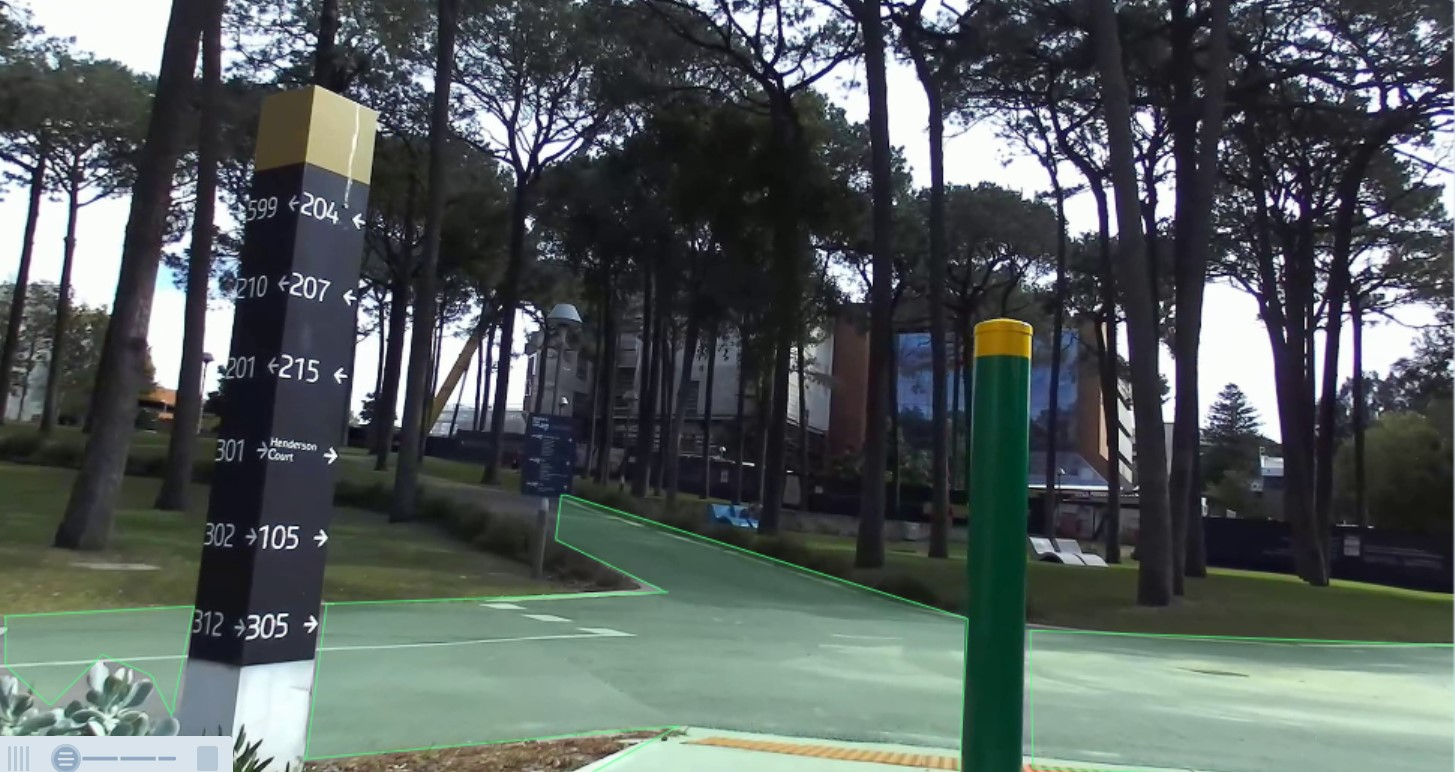
\includegraphics[width=0.8\linewidth]{images/curtin_annotated.jpg}
    \caption{Curtin RGB-D dataset with drivable area annotation}
    \label{fig:curtin_annotated}
\end{figure}
